\section{INCIDENCIAS}
\subsection{Gráfico de dependencias}
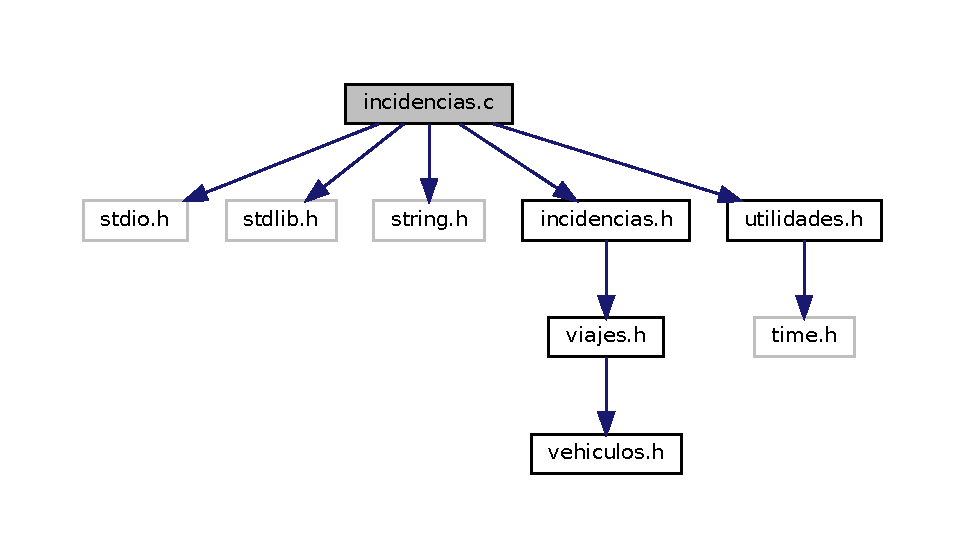
\includegraphics[width=\textwidth, angle=0,scale=0.9]{dep/incidencias_include.pdf}
\subsection{Estructura de Datos}
\begin{itemize}
    \item \funrf{struct Incidencias}{struct:incidencias}
    \item \funrf{struct vIncidencias}{struct:vincidencias}
\end{itemize}
\subsection{Funciones}
\begin{itemize}
    \item \cc{Incidencias* initIncidencias(int *n)}
    \item \cc{void saveIncidencias(int n,Incidencias* incidencias)}
    \item \cc{int incidenciasUsuario(vIncidencias* v,int userId)}
    \item \cc{void listarIncidencias(vIncidencias* v)}
    \item \cc{void crearIncidenciasAdmin(vIncidencias* v,vViajes* vv,vVehiculos* ve)}
    \item \cc{void crearIncidenciasUser(vIncidencias*v,vViajes* vv ,vVehiculos* ve,int userId )}
    \item \cc{void eliminarIncidenciasAdmin(vIncidencias* v,vViajes* vv)}
    \item \cc{void modificarIncidenciasAdmin(vIncidencias* v)}
\end{itemize}
\subsection{Definiciones}
\begin{itemize}
	\item \cc{Incidencias* initIncidencias(int *n)}
	\begin{itemize}
		\item \textbf{Descripción}
        \begin{itemize}
			\item Inicializa las incidencias.
		\end{itemize}
        \item \textbf{Parámetros}
		\begin{itemize}
			\item \cc{n} $\rightarrow$ Índice.
		\end{itemize}
		\item \textbf{Devuelve}
		\begin{itemize}
			\item Incidencias inicializadas.
		\end{itemize}
	\end{itemize}
    \newpage
	\item\cc{void saveIncidencias(int n,Incidencias* incidencias)}
	\begin{itemize}
		\item \textbf{Descripción}
        \begin{itemize}
			\item Guarda las incidencias.
		\end{itemize}
        \item \textbf{Parámetros}
		\begin{itemize}
			\item \cc{n} $\rightarrow$ Índice.
            \item \cc{incidencias} $\rightarrow$ Estructura.
		\end{itemize}
	\end{itemize}
    \item\cc{int incidenciasUsuario(vIncidencias* v,int userId)}
	\begin{itemize}
		\item \textbf{Descripción}
        \begin{itemize}
			\item Devuelve un índice.
		\end{itemize}
        \item \textbf{Parámetros}
		\begin{itemize}
			\item \cc{v} $\rightarrow$ Vector incidencias.
            \item \cc{userId} $\rightarrow$ Identificador del usuario logueado.
		\end{itemize}
        \item \textbf{Devuelve}
		\begin{itemize}
			\item Número de incidencias de un usuario.
		\end{itemize}
	\end{itemize}
    \item\cc{void listarIncidencias(vIncidencias* v)}
	\begin{itemize}
		\item \textbf{Descripción}
        \begin{itemize}
			\item Lista todas las incidencias.
		\end{itemize}
        \item \textbf{Parámetros}
		\begin{itemize}
			\item \cc{v} $\rightarrow$ Vector incidencias.
		\end{itemize}
	\end{itemize}
	\item\cc{void crearIncidenciasAdmin(vIncidencias* v,vViajes* vv,vVehiculos* ve)}
	\begin{itemize}
		\item \textbf{Descripción}
        \begin{itemize}
			\item Función exclusiva para administradores, en la que el administrador logueado puede crear una nueva incidencia.
		\end{itemize}
        \item \textbf{Parámetros}
		\begin{itemize}
			\item \cc{v} $\rightarrow$ Vector incidencias.
            \item \cc{vv} $\rightarrow$ Vector viajes.
            \item \cc{ve} $\rightarrow$ Vector vehículos.
		\end{itemize}
	\end{itemize}
    \item\cc{void crearIncidenciasUser(vIncidencias*v,vViajes* vv ,vVehiculos* ve,int userId )}
	\begin{itemize}
		\item \textbf{Descripción}
        \begin{itemize}
			\item Función exclusiva para usuarios, en la que el usuario logueado puede crear una nueva incidencia.
		\end{itemize}
        \item \textbf{Parámetros}
		\begin{itemize}
            \item \cc{v} $\rightarrow$ Vector incidencias.
            \item \cc{vv} $\rightarrow$ Vector viajes.
            \item \cc{ve} $\rightarrow$ Vector vehículos.
            \item \cc{userId} $\rightarrow$ Identificador del usuario logueado.
		\end{itemize}
	\end{itemize}
    \item\cc{void eliminarIncidenciasAdmin(vIncidencias* v,vViajes* vv)}
	\begin{itemize}
		\item \textbf{Descripción}
        \begin{itemize}
			\item Función para administradores. El administrador logueado puede eliminar una incidencia de la base de datos.
		\end{itemize}
        \item \textbf{Parámetros}
		\begin{itemize}
			\item \cc{v} $\rightarrow$ Vector incidencias.
            \item \cc{vv} $\rightarrow$ Vector viajes.
		\end{itemize}
	\end{itemize}
    \newpage
    \item\cc{void modificarIncidenciasAdmin(vIncidencias* v)}
	\begin{itemize}
		\item \textbf{Descripción}
        \begin{itemize}
			\item Función para administradores. Modifica las incidencias de la base de datos.
		\end{itemize}
        \item \textbf{Parámetros}
		\begin{itemize}
			\item \cc{v} $\rightarrow$ Vector incidencias.
		\end{itemize}
	\end{itemize}
\end{itemize}
\newpage